\section{Results \& Discussion}
\label{sec:results}

We first compare accuracy and total runtime against g2o, then dissect 
per‑iteration trends, and finally analyze two ablations: (a) disabling the T$^{2}$SC 
pipeline and (b) switching to single‑precision arithmetic.

\subsection{Runtime and Accuracy Overview}
\label{subsec:results_runtime}
Table~\ref{tab:results_runtime} summarizes both accuracy ($\chi^{2}$ cost) and wall-clock runtime 
performance. Our solver achieves near-optimal convergence within the 10-iteration budget, with 
final $\chi^{2}$ costs deviating by at most 0.52\% from fully converged values. This rapid 
convergence, combined with our cache-optimized implementation, yields significant speed-ups over 
g2o: 1.2--2.7$\times$ faster on the Cortex-A53 and 2.3--8.8$\times$ faster on the Core i9. The 
speed-up is particularly pronounced on larger problems like Ladybug-3, where our solver completes 
in 1.2s on the i9 compared to g2o's 4.4s.

Beyond raw performance, our solver demonstrates superior numerical stability. G2o struggles with 
convergence on several datasets, most notably Dubrovnik-1 where its final $\chi^{2}$ cost 
(124,093) is 3.4$\times$ higher than our method's (36,068). This validates the effectiveness of 
our parameter scaling and mixed-precision differentiation strategies in maintaining both speed and 
accuracy.

\begin{table*}[t]
\caption{Accuracy and runtime after ten LM iterations. Speed-up is relative to g2o.}
\label{tab:results_runtime}
\centering
\begin{tabular}{@{}lcccccccc@{}}
\toprule
& \multicolumn{4}{c}{\textbf{$\chi^{2}$ after iteration 10}} & \multicolumn{4}{c}{\textbf{Time for 10 iterations [ms]}} \\
\cmidrule(lr){2-5} \cmidrule(lr){6-9}
Dataset & Ours & g2o & Final & \% vs Final & Ours A53 & g2o A53 & Ours i9 & g2o i9 \\
\midrule
Ladybug‑1   & 26700.7 & 30980.5 & 26688.7 & +0.04\% & 3202 & 8601 & 189 & 1662 \\
Dubrovnik‑1 & 36067.7 & 124093.1 & 36067.7 & +0.00\% & 9651 & 17418 & 680 & 1562 \\
Ladybug‑2   & 34288.4 & 34391.6 & 34198.9 & +0.26\% & 7214 & 14561 & 471 & 3000 \\
Trafalgar‑3 & 103754.9 & 141586.9 & 103218.1 & +0.52\% & 9138 & 16999 & 836 & 2159 \\
Ladybug‑3   & 118788.8 & 129259.0 & 118749.2 & +0.03\% & 36325 & 43487 & 1223 & 4433 \\
\bottomrule
\end{tabular}
\end{table*}

% -------------------------------------------------------
\subsection{Per-Iteration Scaling on the Synthetic Suite}
\label{subsec:results_itercost}
Figure~\ref{fig:results_scaling_synth} plots the mean time per
Levenberg–Marquardt (LM) iteration against the number of
$\mathbf Y\mathbf W^{\!\top}$ tiles. Both sweeps—one varying pose count and the other landmark 
count—exhibit a strong linear trend (R$^{2}\!>\!0.98$). This confirms that our tiled two-phase 
Schur (T$^{2}$SC) pipeline scales directly with the \emph{true} computational workload rather 
than abstract graph metrics like vertex or edge counts. A unified linear fit across both 
synthetic series reveals a consistent cost of approximately \SI{0.11}{\micro\second} per 
$\mathbf Y\mathbf W^{\!\top}$ tile on the i9 CPU. This result supports our central claim: 
cache-friendly data organization transforms the workload into a predictable, compute-bound 
problem dominated by matrix multiplication.

\begin{figure}[t]
  \centering
  % Export the PNG/PDF produced by the analysis script to figs/ first.
  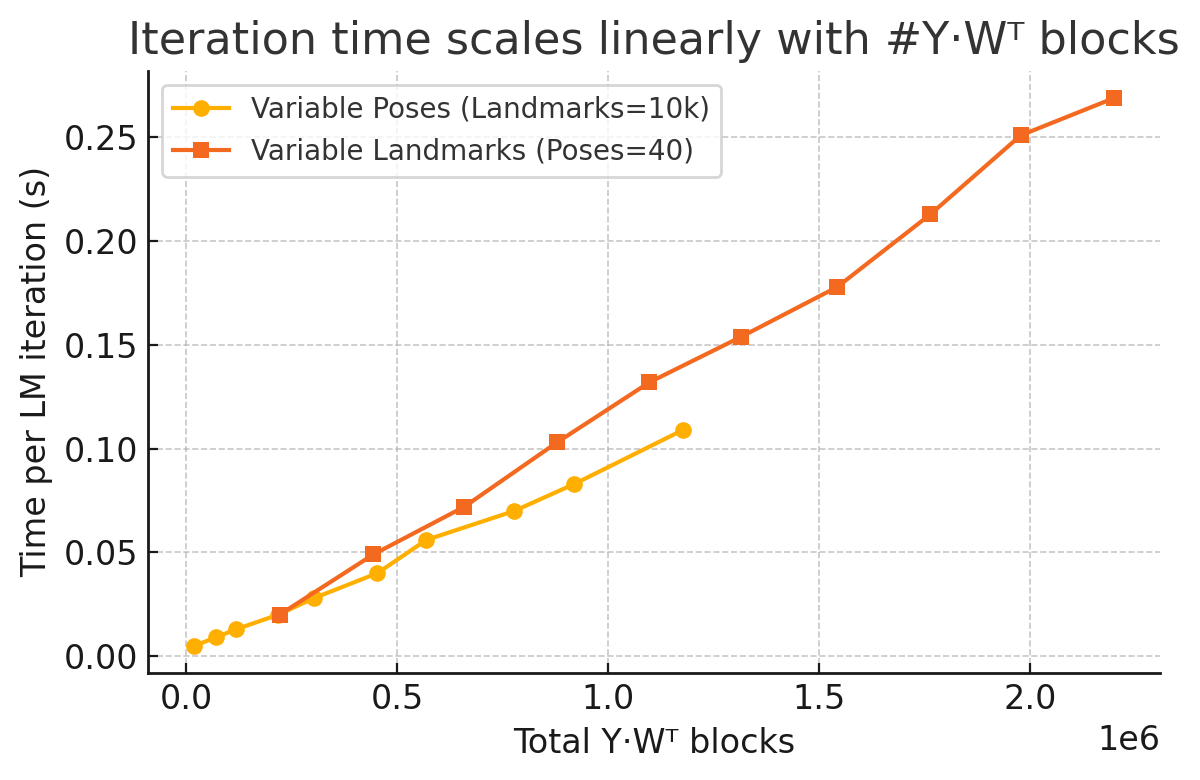
\includegraphics[width=\linewidth]{figs/synth_scaling_YWt}
  \caption{Time per LM iteration on the Core~i9-9900K as a
    function of the number of $\mathbf Y\mathbf W^{\!\top}$ tiles
    in the synthetic scalability suite.  \emph{Circles:} landmarks
    fixed (10 k) while poses increase.  \emph{Squares:} poses fixed
    (40) while landmarks increase. The shared slope
    ($\approx$\SI{0.11}{\micro\second} per tile) indicates that
    $\mathbf{Y}\mathbf{W}^{\!\top}$ multiplication dominates runtime.}
  \label{fig:results_scaling_synth}
\end{figure}

\subsection{Ablation Study}
\label{subsec:results_ablation}
\paragraph{(a) Impact of T\textsuperscript{2}SC.} Table~\ref{tab:ablate_t2sc} shows that disabling 
T$^{2}$SC consistently slows performance on the memory-bandwidth-limited A53 by 2.3–3.2$\times$. 
On the i9, which has a much larger cache, the benefits are even more pronounced on smaller 
problems (up to 12.9$\times$) but diminish as the total tile memory footprint grows. Nonetheless, 
it provided a clear net benefit in all tested scenarios.

\paragraph{(b) Single vs.\ double precision.}  Table~\ref{tab:ablate_precision} confirms that 
float32 reduces memory footprint by 38.9–42.0\% while maintaining $\chi^{2}$ accuracy within 
0.01\% of double‑precision results, with no observable loss in convergence quality.

\begin{table}[h]
\caption{Ablation (a): T$^{2}$SC on/off runtime comparison (ms).}
\label{tab:ablate_t2sc}
\centering
\begin{tabular}{@{}lcccc@{}}
\toprule
& \multicolumn{2}{c}{A53} & \multicolumn{2}{c}{i9} \\
\cmidrule(lr){2-3} \cmidrule(lr){4-5}
Dataset & ON & OFF & ON & OFF \\
\midrule
Ladybug‑1   & 45.6  & 147.3 & 3.9  & 50.4 \\
Dubrovnik‑1 & 184.9 & 315.3 & 22.9 & 96.1 \\
Ladybug‑2   & 82.1  & 238.0 & 6.5  & 78.4 \\
Trafalgar‑3 & 164.2 & 300.1 & 32.5 & 106.0 \\
Ladybug‑3   & 187.8 & 502.0 &  15.3 & 169.0 \\
\bottomrule
\end{tabular}
\end{table}

\begin{table*}[h]
\caption{Ablation (b): float32 vs double precision comparison.}
\label{tab:ablate_precision}
\centering
\begin{tabular}{@{}lccc@{}}
\toprule
Dataset & $\chi^{2}_{\text{f32}}$ & $\chi^{2}_{\text{f64}}$ & RAM \% save \\
\midrule
Ladybug‑1   & 26775.908 & 26783.331 & 38.9\% \\
Dubrovnik‑1 & 36067.785 & 36067.835 & 39.2\% \\
Ladybug‑2   & 34318.758 & 34318.709 & 40.3\% \\
Trafalgar‑3 & 123822.656 & 123820.275 & 39.0\% \\
Ladybug‑3   & 119939.984 & 119940.173 & 42.0\% \\
\bottomrule
\end{tabular}
\end{table*}

\subsection{Peak Memory Consumption}
\label{subsec:results_ram}
Table~\ref{tab:peak_ram} contrasts resident set size across different configurations. 
The T$^{2}$SC pipeline requires 2.1–2.5$\times$ more memory than the baseline version, 
with peak usage reaching \SI{290.4}{MB} on the largest dataset. Interestingly, our baseline 
(T$^{2}$SC off) uses less memory than g2o on most datasets, while the full T$^{2}$SC version 
trades memory for significant speed improvements. Future work will explore tile compression 
and out‑of‑core variants.

\begin{table}[h]
\caption{Peak RAM usage (values in MB).}
\label{tab:peak_ram}
\centering
\begin{tabular}{@{}lccccc@{}}
\toprule
& \multicolumn{5}{c}{Dataset} \\
\cmidrule(lr){2-6}
Implementation & Ladybug-1 & Dubrovnik-1 & Ladybug-2 & Trafalgar-3 & Ladybug-3 \\
\midrule
Ours (+T$^{2}$SC) & 101.7 & 219.2 & 148.5 & 206.0 & 290.4 \\
Ours (-T$^{2}$SC) &  48.0 & 104.2 &  64.6 &  94.9 & 115.8 \\
g2o             &  52.9 &  104.4 &  74.3 &  98.4 & 132.8 \\
\bottomrule
\end{tabular}
\end{table}

\subsection{Discussion and Limitations}
\label{subsec:results_discussion}
The results reveal distinct performance characteristics across platforms. On the i9, the 
large \SI{16}{MB} LLC enables cache‑resident tile processing, delivering 2.3–8.8$\times$ 
speed‑ups over g2o. The effectiveness of T$^{2}$SC varies with problem size; while smaller 
problems see dramatic acceleration (up to 12.9$\times$), the advantage diminishes for larger 
problems as tile memory begins to exceed cache capacity. On the A53 platform, where memory 
bandwidth is the primary bottleneck, T$^{2}$SC provides a consistent and significant 
2.3–3.2$\times$ speed-up. This suggests our contiguous storage and batched BLAS approach is 
highly effective in memory-constrained scenarios. A key limitation is memory overhead: T$^{2}$SC 
requires 2.1–2.5$\times$ more RAM, reaching \SI{290.4}{MB} on the largest dataset—a significant 
constraint for embedded deployment.